\begin{comment}
- \cite{kurth2003experimental}
	- Many tasks for which robots are seemingly well-suited require a high level of precision in localization before such application can occur in the eld. For ex-ample, a robot delivering mail in an oÆce building, moving plants in a greenhouse, or mapping an under-ground mine needs to maintain an accurate estimate of its location.
	- Originally intended as a means to track assets and people in an environment equipped with special RF transponders [13], we invert the paradigm by xing the tags in the environment and moving a transponder with a robot. In this paradigm, as the robot moves, it periodically sends out a query, and any tags within range respond by sending a reply.
	- The ad-vantage of such a method is that it does not require line of sight between tags and the mobile robot, mak-ing it useful in many environmental conditions that fail optical methods.
	- Note that, since each tag transmits a unique ID number, distance readings are automatically associated with the appropriate tags, so the data association problem is solved trivially.
- \cite{djugash2010geolocation}
	- Geolocation with range - Robustness, efficiency and scalability.pdf
	
- \cite{liu2007survey}
	- Survey of wireless indoor positioning techniques and systems (3151)
	- These systems provide a new layer of automation called automatic object location detection. Realworld applications depending on such automation are many. To name a few, one can consider the location detection of products stored in a warehouse, location detection of medical personnel or equipment in a hospital, location detection of firemen in a building on fire, detecting the location of police dogs trained to find explosives in a building, and finding tagged maintenance tools and equipment scattered all over a plant.
	- Wireless technologies have entered the realms of consumer applications, as well as medical, industrial, public safety, logistics, and transport system along with many other applications. Self-organizing sensor networks, location sensitive billing, ubiquitous computing, context-dependent information services, tracking, and guiding are some of the numerous possible application areas. Since wireless information access is now widely available, there is a high demand for accurate positioning in wireless networks, including indoor and outdoor environments [1], [2]. The process of determining a location is called location sensing, geolocation, position location, or radiolocation, if it uses wireless technologies.
	
- \cite{decawave2014rtls}
	- Real time location systems - An Introduction
	- Real Time Location Systems (RTLS) describe a class of Systems that provide information in Real-Time about the Location of objects, animals, people or just about anything you care to imagine.
	- The most pervasive example of an RTLS is GPS.
	- GPS doesn’t work indoors so all the tracking and location functionality that GPS provides suddenly disappears.
	- examine the application of RTLS to specific market areas such as Healthcare, Agriculture and Logistics
	- RTLS USE CASES
		- Proximity
			- This is the simplest form of RTLS where the requirement reduces to the need to determine the distance between two items. Nodes establish how far apart they are from each other and take action accordingly.
			- A mobile phone’s separation from a laptop or other personal possession – the “find my stuff” application. All items involved would need to be DecaWave enabled.
			- The proximity of a key fob to its associated automobile
			- The proximity of an Alzheimer’s patient or infant to an unlocked door through which they are not authorized to pass
		- Absolute Location using Fixed Infrastructure
			- The location of tagged objects is established using a number of fixed anchors in known locations around the area in which the tagged objects are located.
			- These anchors can be separate units or can be incorporated into Wireless Access Points
			- The tracking and location of assets and patients in healthcare
providing:
				 Significantly improved patient care,
				 Increases in efficiency and
				 Reductions in operating costs
			- The tracking and location of pallets, packages and items in warehousing and logistics applications leading to:
				 Reductions in wait time
				 Improved customer service
				 Reduction in operating costs
			- The tracking and monitoring of farm animals leading to:
				 Improvements in animal health and yield
				 Reduction in operating costs
				 The tracking of Inventory, Work in Progress and Finished Goods in manufacturing environments
				 The tracking of which components have been assembled to other components
				 The monitoring of tool movements to ensure manufacturing sequences are carried out in the correct order
		- Relative Location Among a Group of Nodes
			- In this situation there is no fixed infrastructure so nodes must establish their location relative to other nodes in the network.
			- You might find this kind of scenario in first-responder situations, for example, where emergency services arrive at a building that is not equipped with RTLS infrastructure but yet they need to track the progress of their personnel as they enter the building.
			- In order for this information to be available to the command centre, one or more of the first responders will need to be linked wirelessly to the command vehicle outside the building.
			- If absolute location is required then at least two nodes that are in known locations relative to the building are required. These would need to be “dropped” by the first responders or their support crew on arrival at the building and their locations noted
- \cite{decawave2016dw1kusermanual}
	- Infrastructure based asset tracking
		- Each tag can now calculate its distance from the anchor after a sequence of just 7 messages. If the anchor had used symmetric S-TWR it would be forced to have the same delay for each tag interaction and a minimum of 3 messages per tag, or 15 messages would be required.
		- In the asymmetric case the number of packets required is N+2 whereas in the symmetric case it is 3N.
	- Infrastructure based asset tracking
		- In this scheme a mobile tag (on an asset say) ranges to three fixed anchors. Each anchor then calculates the distance to the tag. These three distances are then combined in an infrastructure-based solver to locate the tag.
		- In the asymmetric ranging scheme the tag sends a Poll message which is received by the three anchors in the infrastructure who reply in successive responses with packets RespA, RespB & RespC after which the tag sends the Final message received by all three anchors. This allows the tag to be located after sending only 2 messages and receiving 3. This scheme is illustrated in Figure 39.
		- This represents a substantial saving in message traffic thereby saving battery power and air-time.
	- Infrastructure-less Peer-to-peer networks
	
\end{comment}



\chapter{Einführung [todo]}

Mit dem vorliegenden Artikel sollen die Einsatzmöglichkeiten der seriellen Kommunikation mit Peripheriegeräten mittels \gls{spi} verdeutlicht werden.

Das \gls{spi} ist ein in den frühen 1980er Jahren von Motorola entwickeltes Bus-System mit einem „lockeren“ Standard für einen synchronen seriellen Datenbus (Synchronous Serial Port), mit dem digitale Schaltungen nach dem Master-Slave-Prinzip miteinander verbunden werden können.

\begin{figure}[h]
    \centering
    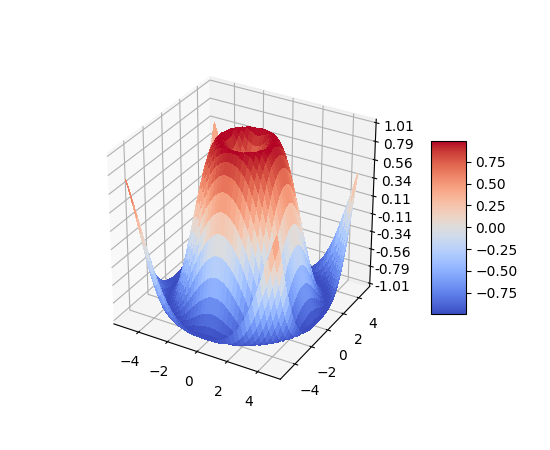
\includegraphics[width=0.25\textwidth]{surface3d_demo4}
    \caption{a nice plot}
    \label{fig:mesh1}
\end{figure}
 
As you can see in the figure \ref{fig:mesh1}, the function grows near 0. Also, in the page \pageref{fig:mesh1} is the same example.

The table \ref{table:1} is an example of referenced \LaTeX elements.
 
%LaTeX Warning: `!h' float specifier changed to `!ht'.
%\begin{table}[h!]
\begin{table}[!ht]
\centering
\begin{tabular}{||c c c c||} 
 \hline
 Col1 & Col2 & Col2 & Col3 \\ [0.5ex] 
 \hline\hline
 1 & 6 & 87837 & 787 \\ 
 2 & 7 & 78 & 5415 \\
 3 & 545 & 778 & 7507 \\
 4 & 545 & 18744 & 7560 \\
 5 & 88 & 788 & 6344 \\ [1ex] 
 \hline
\end{tabular}
\caption{Table to test captions and labels}
\label{table:1}
\end{table}

\section{Aufgabenstellung [todo]}

\section{Motivation [todo]}

\section{Zielsetzung [todo]}

\section{Gliederung [todo]}

\section{???Problemstellung?? [todo]}

In der Zeit vor den Navigationsgeräten wurden auf deutschen Straßen noch regelmäßig faltbare Straßenkarten von den Beifahrern verwendet um den Fahrer den Weg zu weisen. Bevor eine Straßenkarten verwendet werden kann, muss diese Erstellt werden. Dieser Prozess ist unter dem Begriff Kartenerstellung (engl. Mapping) bekannt. Der Detailgrad hängt dabei stark vom Verwendungszweck ab. Der erste Schritt nach dem entfalten der Straßenkarten bestand in der Lokalisierung (engl. Localization), also der Bestimmung der ungefähren Fahrzeugposition und dem Ziel der Reise auf der Straßenkarte. Darauf aufbauend wurde vom Beifahrer dann eine Route zwischen der aktuellen Fahrzeugposition und dem Ziel geplant und während der Fahrt weiter verfolgt, was auch als Pfad-Planung (engl. Path-Planning) bekannt ist.

Genauso wie der menschliche Agent muss auch jeder mobile Roboter für sich diese grundlegende Frage beantworten können. \glqq Wo bin ich?\grqq{}, \glqq Wo bin ich bereits gewesen?\grqq, \glqq Wohin gehe ich?\grqq{} und \glqq Welcher ist der beste Weg dahin?\grqq{}\cite{murphy2000introduction}.

Außerhalb von geschlossenen Räumlichkeiten (engl. Outdoor) erfolgt die Lokalisierung in der Regel mittels GPS, unter der Voraussetzung das eine ungehinderte Verbindung zu den GPS-Satelliten möglich ist. Die Lokalisierung ist in diesem Fall sehr einfach, da die GPS Koordinaten eindeutig sind und das Kartenmaterial bereits im gleichen Koordinatensystem vorliegt.

Innerhalb geschlossener Räumlichkeiten (engl. Indoor), wie in öffentlichen Gebäuden, Logistikhallen oder auch in Bergwerken, ist eine Lokalisierung mittels GPS nicht mehr möglich. Erschwerend kommt dazu, dass es in der Regel zu diesen Räumlichkeiten keine öffentlich verfügbaren Karten gibt oder diese sich wie im letzten Beispiel häufig ändern. Aus diesem Problemfeld haben sich Algorithmen für die Simultane Lokalisierung und Kartenerstellen (engl. Simultaneous Localization and Mapping (SLAM)) entwickelt.

Häufig werden SLAM Algorithmen verwendet um aus Kamerabildern oder \SI{360}{\degree} Abstandsmessungen eine Karte der Umgebung zu erstellen und sich in der gleichen zu lokalisieren. Der Fokus dieser Arbeit liegt jedoch auf den reinen Entfernungsbasieren SLAM (engl. Range Only SLAM (RO--SLAM)) Algorithmen. Hierbei werden nur die Informationen der Eigenbewegung und die Entfernungen zu mehreren, vorher unbekannten, Basisstationen genutzt um sich selbst zu Lokalisieren und eine Karte mit den Positionen der Basisstationen zu erstellen.